\section{Introduction}
We are required to extend the capabilities of an implemented RDT (Reliable Data Transfer) model on the link layer to multiple neighbours.\\

The given implementation functions for a setup of two stations communicating to each other illustrated in figure \ref{fig:originalsetup}.
\begin{figure}[H]
\centering
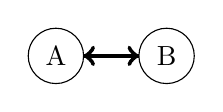
\begin{tikzpicture}

\draw[black] (0,0) circle (10pt) node [anchor=center] {A};
\draw[black] (40pt,0) circle (10pt) node [anchor=center] {B};
\draw[black,ultra thick,->] (10pt,0) -- (30pt,0);
\draw[black,ultra thick,<-] (10pt,0) -- (30pt,0);

\end{tikzpicture}
\caption{Original setup}
\label{fig:originalsetup}
\end{figure}

The extended version of the implementation should work for a fixed number of neighbours, an example of which is given in figure \ref{fig:threestationsetup}, where three stations each have the other two stations as neighbours, which they both send to and receive from.\\

\begin{figure}[H]
\centering
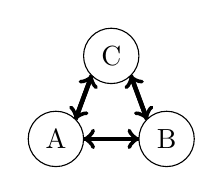
\begin{tikzpicture}

\draw[black] (0,0) circle (10pt) node [anchor=center] {A};
\draw[black] (40pt,0) circle (10pt) node [anchor=center] {B};
\draw[black] (20pt,30pt) circle (10pt) node [anchor=center] {C};

%A<->B
\draw[black,ultra thick,->] (10pt,0) -- (30pt,0);
\draw[black,ultra thick,<-] (10pt,0) -- (30pt,0);

%A<->C
\draw[black,ultra thick,->] (7.07pt,7.07pt) -- (12.92pt,22.92pt);
\draw[black,ultra thick,<-] (7.07pt,7.07pt) -- (12.92pt,22.92pt);

%B<->C
\draw[black,ultra thick,->] (32.92pt,7.07pt) -- (27.06pt,22.92pt);
\draw[black,ultra thick,<-] (32.92pt,7.07pt) -- (27.06pt,22.92pt);

\end{tikzpicture}
\caption{Three station setup}
\label{fig:threestationsetup}
\end{figure}
